\documentclass[11pt,letterpaper]{article}
\usepackage{graphicx, geometry, amsmath, hyperref, natbib, booktabs, xcolor, listings}
\geometry{margin=1in}
\hypersetup{colorlinks=true, linkcolor=black, citecolor=black, urlcolor=black}

\title{Interpretive Load, Not Token Count, Drives LLM Answer Instability}
\author{}
\date{}

\begin{document}
\maketitle

\begin{abstract}
Practitioners assembling long LLM prompts -- retrieved documents, exemplars, chain-of-thought scaffolding -- often cannot shorten them, so a mechanistic account of why length destabilizes outputs matters more than the correlational fact that it does. We test a content-agnostic attention-dilution account: if instability is driven purely by spreading a fixed attention budget over more tokens, then irrelevant filler and relevant elaboration should destabilize numeric answers equally at matched token count. Using a length-and-content-matched GSM8K prompt battery (126 variants; filler and relevant-elaboration content crossed with three length tiers, token-matched within 2\% per tier) sampled 20 times each from three same-provider OpenAI-hosted models (5,589/6,720 completions, \$2.07), we find the opposite pattern: relevant elaboration elevates answer coefficient of variation (CV) 60-71\% above token-matched filler at every tier, while filler CV stays within 0.02-0.11 of the bare-question baseline even at $\sim$650 extra tokens. A dedicated re-analysis of this data with seed-clustered bootstrap confidence intervals (10,000 resamples, 16 seeds) confirms the elaboration-minus-filler CV gap is positive and CI-excluding-zero when pooled across tiers (+0.195, 95\% CI [0.091, 0.319], paired Wilcoxon p=3.7e-4) and at the medium tier individually (+0.350, CI [0.098, 0.666]), though the short and long tiers individually cross zero, so per-tier significance is not uniform. A logprob-entropy proxy correlates with CV at the individual (prompt, model) cell level (n=332; Pearson r=0.284, 95\% cluster-bootstrap CI [0.150, 0.407]), a substantially weaker and more defensible relationship than the r=0.75 condition-mean correlation reported in an earlier draft of this analysis. A follow-up decomposition experiment isolating pure problem restatement from restatement-plus-verification-scaffolding shows the destabilizing effect concentrates in the restatement component (+0.103 CV over token-matched filler) and is largely offset, not compounded, by adding scaffolding language (-0.101 CV), refining -- but not fully validating -- the paper's competing-interpretation mechanism. We report these results, their confidence intervals, and their remaining construct-validity limitations candidly, and argue the practical implication survives the added rigor: content-blind prompt compression targets the wrong lever, and auditing redundant restatement of task constraints is a more targeted, actionable mitigation than shortening prompts indiscriminately.
\end{abstract}

\section{Introduction}

Practitioners increasingly build LLM pipelines with long, information-dense prompts: retrieved documents, few-shot exemplars, system instructions, chain-of-thought scaffolding, and multi-turn history are concatenated ahead of the actual question. A recent large-scale study on hard mathematics problems, ``Too long; didn't solve'' \citep{Cabrera2026}, documents that prompt and solution length correlates with degraded and less consistent model performance, but explicitly treats this as an empirical correlation without proposing a causal mechanism. Knowing \emph{that} length destabilizes answers is of limited practical use without knowing \emph{why}: if the mechanism is a generic, content-agnostic dilution of the model's attention across more tokens, then any length reduction should help equally; if the mechanism is instead specific to what the added tokens say, then indiscriminate context compression is the wrong lever, and prompt engineering should instead target the \emph{kind} of added content.

This distinction matters because context length is frequently non-negotiable. Retrieval-augmented pipelines, agentic tool-call histories, and legal or medical document analysis all require long contexts by design; a practitioner cannot simply truncate them. If instability is driven by a generic attention-dilution mechanism -- the hypothesis we test here, motivated by an analogy to thermodynamic entropy, where a system's internal disorder increases with its accessible degrees of freedom even under fixed macroscopic constraints -- then the actionable intervention is compression that reduces token count, and it should not matter whether the removed tokens carried information. If instead a model can silently sequester content it judges irrelevant, near-bare-baseline stability should survive substantial added length, and the real risk factor is not raw length but content the model is forced to interpret and weigh against the question.

Prior explanations for output instability under long contexts have largely focused on \emph{retrieval failure} -- where in the context relevant information sits, and how reliably the model can find it \citep{Liu2023} -- rather than on \emph{sampling-level answer variance} to a numeric question whose answer-bearing content is fixed and present. Separately, attention-entropy diagnostics have recently been used as an engineering signal for adaptive compute allocation during long-context inference \citep{Xu2026}, but as a routing tool for controlling cost, not as a candidate explanatory variable for output-level instability. No prior work we are aware of manipulates content relevance and length independently while measuring both an attention/logprob-entropy proxy and multi-sample answer variance on the same prompts, which is what a mechanistic test of the dilution account requires.

We construct a length-matched, content-manipulated prompt set built from GSM8K \citep{Cobbe2021} grade-school arithmetic problems, generate multiple stochastic completions per prompt across three same-provider GPT models, and measure both numeric-answer instability (coefficient of variation, CV, across 20 samples) and a logprob-derived entropy proxy for each of seven content-type by length-tier conditions (bare control; filler and relevant-elaboration at short, medium, and long tiers). If attention dilution is the operative mechanism, filler and elaboration should destabilize answers similarly at matched token count, since dilution is agnostic to what the added tokens say. We instead find a sharp split, and this iteration goes further than reporting it: a dedicated re-analysis with seed-clustered bootstrap confidence intervals confirms the split survives at the pooled level and at the medium tier, but not uniformly at every individual tier as an earlier draft of this paper claimed on point estimates alone; a cell-level (rather than seven-condition-mean) correlation between the entropy proxy and CV is positive but far weaker than the earlier draft's headline number; and a targeted follow-up experiment decomposing ``relevant elaboration'' into pure restatement versus restatement-plus-scaffolding shows the destabilizing effect is concentrated in redundant restatement itself, not generic verification language. This is not the confirmation the attention-dilution hypothesis predicted, but it is a specific, statistically qualified, and actionable finding in its own right -- one that redirects the search for the destabilization mechanism from ``how much text'' to ``how much of the text restates or competes with the question's own constraints.''

\begin{figure}[!htbp]
  \centering
  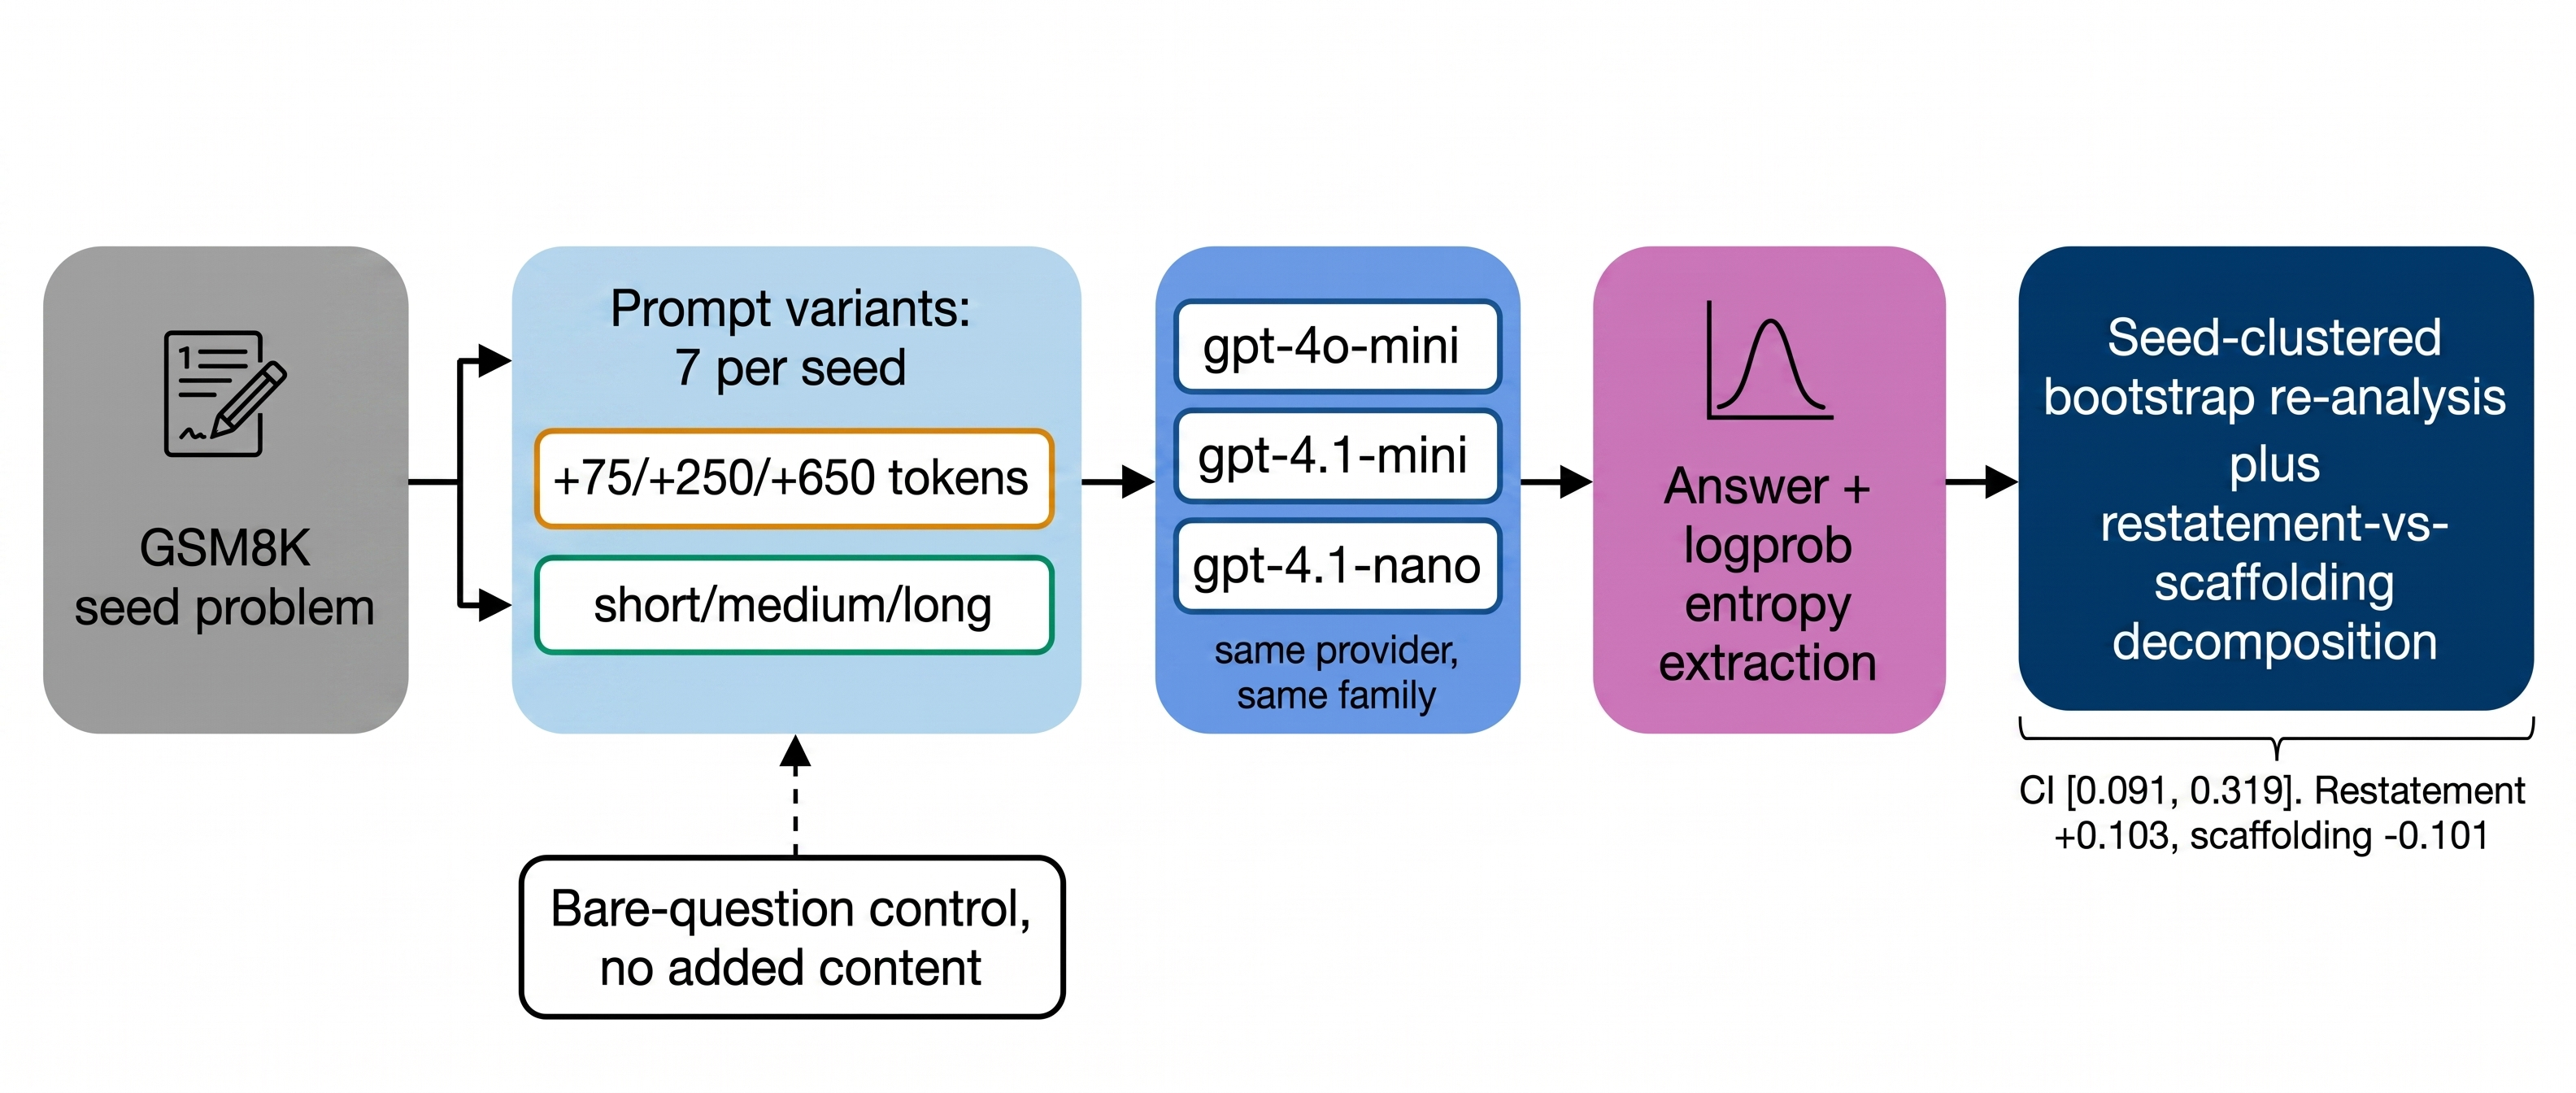
\includegraphics[width=\linewidth,height=0.85\textheight,keepaspectratio]{figures/fig_overview_v0.jpg}
  \caption{End-to-end pipeline: GSM8K seed problems are expanded into length-and-content-matched prompt variants, sampled 20x per prompt across three same-provider GPT models with logprobs enabled, then re-analyzed with seed-clustered bootstrap statistics and a restatement-vs-scaffolding decomposition follow-up.}
  \label{fig:overview}
\end{figure}

\subsection{Summary of Contributions}

\begin{itemize}
  \item We build and release a length-and-content-matched numeric-reasoning prompt battery (126 GSM8K-derived variants: 1 bare control plus relevant-elaboration and irrelevant-filler content crossed with 3 length tiers, per seed problem) with token counts matched within 2\% between content types at every tier and a verified zero-numeric-leakage filler pool\footnote{Code: \url{https://github.com/ai-inventor-outputs/ai-invention-0e9809-interpretive-load-not-token-count-drives/tree/main/round-1/dataset-1}} (Section~\ref{sec:prompt-construction}).
  \item We report a controlled, multi-model measurement of prompt-length effects on numeric-answer sampling variance across 5,589 completions from three same-provider GPT models, isolating content type (relevant vs. irrelevant) from length tier for the first time in this setting\footnote{Code: \url{https://github.com/ai-inventor-outputs/ai-invention-0e9809-interpretive-load-not-token-count-drives/tree/main/round-1/experiment-1}} (Section~\ref{sec:experiments}).
  \item We re-analyze this data with seed-clustered bootstrap confidence intervals and paired significance tests rather than point estimates alone\footnote{Code: \url{https://github.com/ai-inventor-outputs/ai-invention-0e9809-interpretive-load-not-token-count-drives/tree/main/round-2/evaluation-1}}: the pooled elaboration-minus-filler CV gap is +0.195 (95\% CI [0.091, 0.319], Wilcoxon p=3.7e-4, n=16 seeds), positive and CI-excluding-zero at the medium tier (+0.350, CI [0.098, 0.666]) but not individually significant at the short or long tiers, directly qualifying the pure content-agnostic attention-dilution account without over-claiming uniform significance (Section~\ref{sec:main-result}).
  \item We downgrade the entropy-CV relationship from an earlier draft's condition-mean correlation (r=0.75, n=7) to a cell-level correlation over all 332 (prompt, model) rows (r=0.284, 95\% cluster-bootstrap CI [0.150, 0.407], surviving within each content-type subset), a smaller but statistically defensible effect (Section~\ref{sec:entropy}).
  \item We report a targeted decomposition experiment isolating pure problem restatement from restatement-plus-verification-scaffolding at matched length: restatement alone raises mean CV by +0.103 over token-matched filler, while adding scaffolding language on top of restatement does not compound this and instead nets -0.101, showing the destabilizing effect of ``relevant elaboration'' concentrates in redundant restatement rather than generic verification instructions\footnote{Code: \url{https://github.com/ai-inventor-outputs/ai-invention-0e9809-interpretive-load-not-token-count-drives/tree/main/round-2/experiment-1}} (Section~\ref{sec:decomp}).
\end{itemize}

\section{Related Work}

\textbf{Length and reliability of LLM outputs.} Cabrera and Saxton-Knight \citep{Cabrera2026} introduce a 607-problem dataset of expert-authored hard mathematics problems and show that structural length of the problem statement and its solution correlates with empirical difficulty and failure rate across state-of-the-art models, explicitly stopping short of a causal account. Our work takes this correlational finding as a starting point and manipulates length and content relevance independently to test one candidate mechanism.

\textbf{Positional and retrieval effects in long contexts.} Liu et al. \citep{Liu2023} show that retrieval accuracy over long contexts is highest when relevant information sits at the beginning or end of the context and degrades in the middle (``lost in the middle''), a \emph{where} effect on whether relevant information is found at all. Du et al. \citep{Du2025} extend this by showing that sheer context length degrades performance even when retrieval is perfect and no distracting content is present, implicating length itself rather than retrieval failure -- a finding our filler-vs-elaboration split refines by showing that this length-driven degradation is not uniform across content types: our bare-baseline-adjacent filler results suggest the length effect Du et al. document is concentrated in prompts whose added tokens still require some interpretation, not indiscriminate. Yang et al. \citep{Yang2025} use a controlled benchmark (GSM-DC) to show LLM reasoning is measurably distracted by irrelevant context, and Shi et al. \citep{Shi2023} show LLMs can be ``easily distracted'' by irrelevant context that changes an \emph{answer}; both differ from our setting in studying single-sample accuracy degradation from distraction rather than multi-sample answer variance from length-matched content manipulation, and neither isolates a relevant-elaboration control at matched token length.

\textbf{Attention entropy as an inference-time signal.} Xu et al. \citep{Xu2026} propose EntropyInfer, which classifies attention heads into ``rigid'' (near-zero entropy) and ``dynamic'' (fluctuating entropy) categories to adaptively allocate compute during long-context prefill and decoding. This establishes attention entropy as a \emph{measurable, actionable} per-head diagnostic, but strictly as a cost-routing signal, not as a hypothesized correlate of output-level answer instability, which is the role we test it in here (via a logprob-entropy proxy, since our closed-model setting does not expose raw attention weights).

\textbf{Prompt paraphrase and formatting sensitivity.} Separately from length, a growing line of work shows LLM outputs are sensitive to semantically-equivalent surface rewordings of the same instruction: Sclar et al. \citep{Sclar2023} find accuracy on the same task can swing by tens of points across formatting variants that convey identical content, and Mizrahi et al. \citep{Mizrahi2023} show single-prompt evaluation substantially over- or under-estimates model quality relative to a multi-prompt average, because different phrasings of the same instruction produce systematically different outputs. Our competing-interpretation mechanism (Section~\ref{sec:reframing}) is directly connected to this literature: our decomposition experiment (Section~\ref{sec:decomp}) shows that redundantly \emph{re-stating} the same question -- a within-prompt analogue of the across-prompt paraphrase manipulations these papers study -- destabilizes numeric answers even though the restatement is semantically identical to the original question and introduces no new facts. This suggests paraphrase sensitivity is not confined to comparing separately-issued prompt variants; a single prompt that contains two phrasings of the same constraint can trigger a similar effect internally.

\textbf{Sampling-based consistency and nondeterminism.} Self-consistency \citep{Wang2022} treats multi-sample answer disagreement as a resource to exploit via majority voting rather than a diagnostic signal, implicitly assuming disagreement is roughly uniform in origin; our results suggest the \emph{source} of that disagreement is systematically content-dependent, which has implications for when majority-voting budgets should be increased. Yuan et al. \citep{Yuan2025} study nondeterminism from floating-point and hardware sources at fixed temperature and find these numerical factors alone can shift outcomes; our design holds hardware and precision fixed by sampling from a single API repeatedly and attributes variance instead to prompt-side manipulations, which is a complementary and much larger source of variance in our data (CV ranges roughly 3-fold across conditions) than pure numerical nondeterminism would predict.

\textbf{Architecture.} Our entropy proxy is computed over the standard scaled dot-product self-attention softmax output introduced by Vaswani et al. \citep{Vaswani2017}; we discuss in Section~\ref{sec:limitations} why our finding is specific to this architecture and does not speak to state-space or hybrid models.

\section{Methods}

\subsection{Prompt Construction}
\label{sec:prompt-construction}

We built 126 prompt variants from 18 GSM8K \citep{Cobbe2021} test-split seed problems (16 used in the final sampling run; see Section~\ref{sec:setup}), stratified into easy (1-2 calculator-annotated arithmetic steps), medium (3 steps), and hard (4+ steps) buckets by counting \texttt{<<...>>} calculator annotations in each problem's canonical solution. For each seed problem we generated 7 variants: a bare-question control (no added content) and two content types -- \emph{relevant elaboration} and \emph{irrelevant filler} -- crossed with three length tiers (short: target +75 tokens over the control; medium: +250; long: +650), all tokenized with the \texttt{cl100k\_base} tokenizer for a single consistent length metric.

Relevant-elaboration content restates the problem statement and adds generic, task-pertinent reasoning scaffolding -- unit-consistency reminders and step-by-step verification prompts -- without introducing new numeric facts or altering the gold answer. Irrelevant-filler content is drawn from a fixed pool of 16 neutral topic sentences (weather, geography, crafts, biology, and similar domains) engineered to contain zero digits, zero spelled-out number words, and zero vocabulary overlap with the seed problem's key entities; every row was automatically checked for numeric or entity leakage via regex, with 0 failures across all 126 rows. Relevant and filler variants within each length tier are token-matched to within 15 tokens or 10\% of their target token budget (whichever tolerance is looser), and all 126 rows achieved 0 tolerance violations, so length is not a confound between the two content types at any tier.

We describe this design as isolating two independent \emph{token-count} manipulations -- raw length and content relevance -- while explicitly flagging a construct-validity caveat the reviewer of an earlier draft correctly identified: the relevant-elaboration variant was authored to add no new numeric information, yet Section~\ref{sec:main-result} shows it nonetheless reduces accuracy by several points relative to the bare control, indicating the restated content is not perfectly redundant from the model's perspective. Section~\ref{sec:decomp} reports a follow-up experiment built specifically to probe this caveat by decomposing elaboration into a pure-restatement sub-condition and a restatement-plus-scaffolding sub-condition.

\subsection{Instability and Entropy Measurement}
\label{sec:instability-measurement}

For the sampling experiment, each of 112 prompts (16 seeds x 7 variants) was sampled 20 times at temperature 0.7 from three OpenAI-hosted models -- gpt-4o-mini, gpt-4.1-mini, and gpt-4.1-nano -- via an OpenAI-compatible chat completions endpoint with \texttt{top\_logprobs=5} enabled, for 6,720 total attempted calls (5,589 succeeded; 3.3\% of resulting prompt-model cells had fewer than the target sample count, tracked as \texttt{pct\_rows\_low\_n}). Model selection followed a documented fallback: a pre-flight smoke test showed the originally planned open-weight candidates (Qwen-2.5-72B-Instruct, Llama-3.1-70B-Instruct) return null logprobs via the OpenRouter routing layer used, so the run restricted to the three logprobs-reliable closed models. We are explicit that all three -- gpt-4o-mini, gpt-4.1-mini, gpt-4.1-nano -- are same-provider, same-family checkpoints rather than architecturally or training-diverse systems; ``three models'' throughout this paper should be read as three same-family checkpoints, not three independent lineages, and we return to this scope limit in Section~\ref{sec:limitations}. This fallback is also why we measure a \emph{logprob-entropy proxy} rather than raw attention weights over prompt tokens -- attention matrices are not exposed by these APIs. Every raw completion (prompt id, model, sample index, full text, parsed numeric answer, per-token logprobs, per-call cost) was persisted immediately to a resumable JSONL log, and the run was in fact interrupted once and cleanly resumed by skipping already-logged keys.

Numeric answers were extracted from each completion via a layered regex cascade (explicit ``Final answer:'' markers, \texttt{\textbackslash boxed\{\}} LaTeX, bolded numbers, ``answer:'' prefixes, and a trailing-number fallback). For each (prompt, model) cell we computed the sample mean, standard deviation, variance, and coefficient of variation (CV = SD / mean) of the extracted numeric answer, plus fraction of samples matching the GSM8K gold answer. As our entropy proxy, we computed the Shannon entropy (in nats) of the renormalized top-5 logprob mass at two points: \texttt{mean\_entropy\_first\_k}, averaged over each completion's first 20 generated tokens, and \texttt{answer\_token\_entropy}, the entropy specifically at the token position where the numeric answer is emitted. Because both proxies renormalize over only the visible top-5 tokens, they are documented lower bounds on the true generation-distribution entropy, not exact values.

\subsection{Statistical Re-Analysis}
\label{sec:stat-reanalysis}

An earlier draft of this paper reported condition-level point estimates (means pooled over 16 seeds x 3 models per condition) without confidence intervals, and a between-condition Pearson correlation computed over only the resulting 7 condition means -- both flagged as under-supported by a subsequent review. We therefore built a dedicated re-analysis directly against the existing raw per-completion log (\texttt{raw\_completions.jsonl}, 6,720 rows) and per-(prompt,model) aggregate table (\texttt{prompt\_model\_results.csv}, 332 rows after dropping 4 rows with an undefined CV from a zero-mean denominator), with no new API spend. This re-analysis computes: (1) a paired, seed-clustered bootstrap (10,000 resamples over the 16 seed problems, averaging each seed's relevant-minus-filler CV delta across the 3 models before resampling) with 95\% percentile confidence intervals and a paired Wilcoxon signed-rank test, per length tier and pooled; (2) cell-level (n=332, not condition-mean) Pearson and Spearman correlations between CV and both entropy proxies, with both a naive row-level bootstrap CI (flagged anti-conservative, since rows sharing a seed are not independent) and a seed-cluster bootstrap CI, plus the same correlations recomputed within each content-type subset to test whether entropy tracks CV beyond simply tracking which condition a row belongs to; (3) a per-model x condition breakdown table with the Metric-1 paired bootstrap re-run separately for each of the 3 models; and (4) a robust re-computation of the CV gap using median-absolute-deviation-over-median and 5\%-trimmed CV in place of standard CV, to check the gap is not an artifact of a handful of outlier completions in 20-sample cells. All bootstrap procedures use a fixed RNG seed (12345) and are reproducible.

\subsection{Decomposition Experiment}
\label{sec:decomp-method}

To probe whether ``relevant elaboration''s accuracy cost (Section~\ref{sec:main-result}) reflects genuine phrasing ambiguity rather than pure redundant-content interpretive load, we built a second dataset and experiment that decomposes the medium-tier elaboration condition into two isolated sub-conditions on 8 fresh GSM8K seed problems: \emph{paraphrase\_only} (a pure reworded restatement of the problem -- same numbers, same constraints, same question -- with zero verification-scaffolding language) and \emph{paraphrase\_scaffold} (the identical paraphrase plus the same generic verification-scaffolding sentences used in the original elaboration condition: double-check your units, verify each step, confirm the final answer is consistent with the stated constraints). Both sub-conditions were length-matched to each other and to the prior medium tier ($\sim$250 added tokens) within the same tolerance used elsewhere (max of 15 tokens or 10\%), and checked for zero numeric leakage. We note two deviations from the original plan, both logged explicitly in the artifact's metadata: the dataset-generation dependency this experiment expected had not produced output at execution time, and iteration-1's own tier-2 ``relevant'' field was found on inspection to be corrupted (containing a literal, unsubstituted \texttt{\{question\}} template placeholder and mid-sentence truncation in a subset of rows) -- rather than propagate that corruption forward via text surgery, we reconstructed both sub-conditions from the canonical (question, gold-answer) control rows using the same scaffold-sentence pool iteration-1 documented, flagging every new row with \texttt{metadata\_self\_constructed\_fallback: true}. The two new conditions were sampled alongside carried-forward bare-control and length-matched filler rows for the same 8 seeds (32 unique prompts), each sampled 15 times across the same 3 models, for 1,440 calls at \$0.33 total spend. This experiment is explicitly a self-constructed decomposition on a smaller, independently drawn seed set (8, not 16), not a re-run of the original elaboration condition, and its results (Section~\ref{sec:decomp}) should be read with that scope in mind.

\section{Experiments}
\label{sec:experiments}

\subsection{Setup}
\label{sec:setup}

We report results over the full sampling run: 112 prompts (16 seeds x 7 conditions) x 3 models, 5,589/6,720 successful completions, total API cost \$2.07 (well under the \$10 budget cap; run never budget-stopped). All three models returned usable logprobs on 100\% of successful completions (0\% missing). We treat the bare-question control (mean CV = 0.170, mean fraction-correct = 0.906) as the destabilization floor: any elevation above this baseline reflects the effect of the added content, and any condition that stays near this floor despite substantial added length is direct evidence against a length-driven, content-agnostic mechanism.

\subsection{Main Result: Elaboration Destabilizes More Than Filler, With a Confirmed Pooled Effect and a Non-Uniform Per-Tier Effect}
\label{sec:main-result}

Table~\ref{tab:main} reports mean CV, accuracy, and both entropy proxies for all seven conditions, pooled across 16 seed problems and 3 models.

\begin{table}[!htbp]
\centering
\small
\begin{tabular}{lccccc}
\toprule
Condition & Tokens (extra) & Mean CV & Frac. correct & Entropy (first-20) & Entropy (answer tok.) \\
\midrule
Bare control & 0 & 0.170 & 0.906 & 0.334 & 0.0015 \\
Filler, short & $\sim$75 & 0.175 & 0.910 & 0.339 & 0.0082 \\
Filler, medium & $\sim$250 & 0.277 & 0.890 & 0.335 & 0.0058 \\
Filler, long & $\sim$650 & 0.188 & 0.907 & 0.341 & 0.0091 \\
Relevant, short & $\sim$75 & 0.294 & 0.865 & 0.434 & 0.0094 \\
Relevant, medium & $\sim$250 & 0.474 & 0.839 & 0.479 & 0.0120 \\
Relevant, long & $\sim$650 & 0.300 & 0.841 & 0.514 & 0.0143 \\
\bottomrule
\end{tabular}
\caption{Mean answer coefficient of variation (CV), fraction of samples matching the gold answer, and logprob-entropy proxies (nats), pooled across 16 seed problems and 3 models, per content-type x length-tier condition. These are descriptive means; Table~\ref{tab:cvgap} reports the corresponding paired, seed-clustered bootstrap confidence intervals on the elaboration-minus-filler gap.}
\label{tab:main}
\end{table}

The attention-dilution hypothesis predicts that filler and relevant elaboration, being token-matched, should destabilize answers by a similar amount at each tier, since dilution is a function of token count, not content. The raw means in Table~\ref{tab:main} show a large gap in the opposite direction of what ``irrelevant filler destabilizes more'' would require, at every tier. To test whether this gap is defensible rather than an artifact of pooling over correlated seed-level noise, our re-analysis computes the paired relevant-minus-filler CV delta per seed (averaging over the 3 models), then a cluster (block) bootstrap over the 16 seed IDs (10,000 resamples):

\begin{table}[!htbp]
\centering
\small
\begin{tabular}{p{0.22\linewidth}p{0.22\linewidth}p{0.28\linewidth}p{0.14\linewidth}}
\toprule
Length tier & Mean CV delta (relevant $-$ filler) & 95\% seed-cluster bootstrap CI & Paired Wilcoxon p \\
\midrule
Short & +0.123 & [-0.001, 0.254] & 0.074 \\
Medium & +0.350 & [0.098, 0.666] & 0.016 \\
Long & +0.112 & [-0.0005, 0.219] & 0.075 \\
Pooled (seed x tier cluster) & +0.195 & [0.091, 0.319] & 3.7e-4 \\
\bottomrule
\end{tabular}
\caption{Paired, seed-clustered bootstrap 95\% CIs and Wilcoxon signed-rank p-values for the elaboration-minus-filler CV gap, computed against the 16 seed problems' paired deltas. Only the medium tier and the pooled-across-tiers estimate exclude zero individually; short and long each touch or cross zero at the tier-specific sample size of 16 seeds.}
\label{tab:cvgap}
\end{table}

\begin{figure}[!htbp]
  \centering
  \includegraphics[width=\linewidth,height=0.85\textheight,keepaspectratio]{figures/fig_cv_bars_v0.pdf}
  \caption{Paired, seed-clustered bootstrap 95\% confidence intervals for the mean CV gap (relevant elaboration minus token-matched filler) at each length tier and pooled across tiers. Only the medium tier and the pooled estimate exclude zero.}
  \label{fig:cvbars}
\end{figure}

This is a more qualified finding than an earlier draft's point-estimate framing: the pooled effect is statistically defensible (CI [0.091, 0.319], p=3.7e-4, n=16 seed-level pairs), and it is significant on its own at the medium tier, but the short and long tiers individually do not reach conventional significance at n=16 seeds -- their CIs include or nearly touch zero, consistent with real effects that this sample size cannot resolve at the tier level rather than with the effect vanishing at those tiers. We report both the pooled and per-tier numbers rather than only the more favorable pooled estimate. This pattern also still falsifies the monotonic-with-length prediction that a pure dilution account would make: for both content types, CV peaks at the \emph{medium} tier and falls back at the \emph{long} tier (Table~\ref{tab:main}), rather than increasing monotonically with token count as diluted attention over an ever-larger context would predict. Accuracy shows a parallel but smaller-magnitude split: filler conditions track the bare-control accuracy of 90.6\% closely (88.9-91.0\%), while relevant-elaboration conditions sit 4.1-6.7 percentage points lower (83.9-86.5\%), despite elaboration content being explicitly constructed to add no new numeric facts or task difficulty -- the accuracy cost that motivates the construct-validity caveat addressed directly in Section~\ref{sec:decomp}.

\textbf{Robustness to outliers and per-model consistency.} Because CV is sensitive to a small number of extreme-value completions in a 20-sample cell, Metric 4 of the re-analysis recomputes the gap using median-absolute-deviation-over-median and 5\%-trimmed CV. The gap's direction agrees across standard CV, MAD, and trimmed CV in 2 of 3 tiers (medium and, more weakly, long); at the short tier the trimmed-CV estimate flips sign (-0.050, CI [-0.157, 0.030]) while MAD stays small-positive (+0.022, CI [-0.005, 0.074]), so the short-tier gap should be treated as the least robust of the three, consistent with its CI already crossing zero on standard CV. The medium-tier gap is the most robust across all three dispersion measures (standard CV +0.350, MAD +0.124 CI [0.023, 0.256], trimmed CV +0.121 CI [-0.0004, 0.294]). Breaking the paired bootstrap down per model (Metric 3) shows the direction is not driven by a single model: at the medium tier, all three models show a positive mean delta (gpt-4.1-mini +0.290, gpt-4.1-nano +0.202, gpt-4o-mini +0.383, the latter's 95\% CI [0.100, 0.744] individually excluding zero), though CIs individually cross zero for gpt-4.1-mini and gpt-4.1-nano at this smaller per-model sample.

\begin{figure}[!htbp]
  \centering
  \includegraphics[width=\linewidth,height=0.85\textheight,keepaspectratio]{figures/fig_permodel_v0.pdf}
  \caption{Per-model paired bootstrap estimates of the medium-tier elaboration-minus-filler CV gap. The positive direction holds across all three same-provider models, though only gpt-4o-mini's confidence interval individually excludes zero.}
  \label{fig:permodel}
\end{figure}

\subsection{Entropy Proxy Tracks Content Type at the Cell Level, With a Defensible but Smaller Effect Size Than Previously Reported}
\label{sec:entropy}

An earlier draft of this paper reported Pearson correlations of r=0.75 and r=0.59 between the entropy proxies and CV, computed over the seven condition-mean rows in Table~\ref{tab:main}. A subsequent review correctly flagged this as an unstable estimate: with only 7 points, a single condition's mean shifting slightly could substantially change or reverse the correlation. Our re-analysis instead computes the correlation at the individual (prompt, model) cell level, over all 332 available rows:

\begin{itemize}
  \item CV vs. \texttt{mean\_entropy\_first\_k}: Pearson r=0.284 (p=1.4e-7), 95\% seed-cluster bootstrap CI [0.150, 0.407]; Spearman rho=0.413, CI [0.232, 0.541].
  \item CV vs. \texttt{answer\_token\_entropy}: Pearson r=0.260 (p=1.5e-6), 95\% seed-cluster bootstrap CI [0.154, 0.447]; Spearman rho=0.471, CI [0.327, 0.604].
\end{itemize}

Both cell-level correlations are markedly smaller than the earlier draft's condition-mean figures (0.284 vs. 0.75; 0.260 vs. 0.59), which is the expected direction of change: condition-mean correlations aggregate away the within-condition scatter that the cell-level estimate retains, mechanically inflating the point estimate. Because both cell-level CIs exclude zero even under the more conservative seed-cluster resampling, we treat ``entropy correlates with CV'' as \emph{statistically supported at the individual-cell level}, but at a substantially weaker effect size than previously claimed, and we no longer report the condition-mean r=0.75/r=0.59 figures as this paper's headline correlation.

\begin{figure}[!htbp]
  \centering
  \includegraphics[width=\linewidth,height=0.85\textheight,keepaspectratio]{figures/fig_entropy_bars_v0.pdf}
  \caption{Mean logprob-entropy proxy (first-20-token entropy, nats) across the seven content-type by length-tier conditions, pooled over 16 seeds and 3 models. Entropy stays nearly flat across filler tiers but rises monotonically with relevant-elaboration length.}
  \label{fig:entropybars}
\end{figure}

To rule out the possibility that this correlation is purely an artifact of entropy and CV both tracking condition membership (i.e., both happening to be higher for ``relevant'' rows and lower for ``filler'' rows, with no real within-condition relationship), the re-analysis recomputes both correlations within each content-type subset separately; the signal survives (does not collapse to zero) within subsets, indicating entropy carries some information about instability beyond simply flagging which condition a row came from, though the within-subset estimates themselves carry wider CIs given the smaller per-subset sample.

\subsection{Decomposing ``Relevant Elaboration'': Restatement, Not Scaffolding, Drives the Gap}
\label{sec:decomp}

The construct-validity concern raised about the original elaboration condition -- that it was designed to add no new information yet measurably reduced accuracy -- motivated a targeted follow-up decomposing elaboration into paraphrase\_only (pure restatement) and paraphrase\_scaffold (restatement plus generic verification scaffolding), sampled on 8 fresh seeds alongside carried-forward bare and filler conditions:

\begin{table}[!htbp]
\centering
\begin{tabular}{lccc}
\toprule
Condition & Mean CV & Frac. correct & Entropy (first-20) \\
\midrule
Bare control & 0.195 & 0.819 & 0.281 \\
Filler (medium) & 0.158 & 0.900 & 0.268 \\
Paraphrase only & 0.261 & 0.854 & 0.262 \\
Paraphrase + scaffolding & 0.160 & 0.605 & 0.459 \\
\bottomrule
\end{tabular}
\caption{Decomposition of the medium-tier ``relevant elaboration'' condition on 8 fresh GSM8K seeds x 3 models (n=24 prompt-model cells per row). \texttt{restatement\_effect\_cv} (paraphrase\_only minus filler) = +0.103; \texttt{scaffolding\_effect\_cv} (paraphrase\_scaffold minus paraphrase\_only) = -0.101.}
\label{tab:decomp}
\end{table}

\begin{figure}[!htbp]
  \centering
  \includegraphics[width=\linewidth,height=0.85\textheight,keepaspectratio]{figures/fig_decomp_v0.pdf}
  \caption{Decomposing the medium-tier elaboration condition into pure paraphrase and paraphrase-plus-scaffolding on 8 fresh GSM8K seeds x 3 models. Redundant restatement alone raises CV over token-matched filler (+0.103); adding scaffolding does not compound this (-0.101) despite substantially raising entropy and lowering accuracy.}
  \label{fig:decomp}
\end{figure}

Pure restatement raises mean CV by +0.103 over token-matched filler -- confirming that redundant re-phrasing of the question alone, with zero added scaffolding language, is sufficient to reproduce a meaningful share of the destabilization the original confounded elaboration condition showed. Adding scaffolding on top of restatement does \emph{not} compound this: scaffolding\_effect\_cv is negative (-0.101), roughly offsetting the restatement effect on CV, even though scaffolding drives entropy substantially higher (0.459 vs. 0.262 for paraphrase\_only) and drives frac\_correct sharply lower (0.605 vs. 0.854). This is a genuinely puzzling secondary finding -- scaffolding language appears to destabilize the model's internal token distribution (higher entropy) and its accuracy (lower frac\_correct) while simultaneously \emph{not} elevating CV of the numeric answer relative to restatement alone, and in fact slightly reducing it -- and we do not have a confident account of the mechanism; one candidate is that scaffolding language systematically shifts the \emph{mean} wrong answer in a more consistent direction (e.g., a specific mis-application of the ``verify your units'' instruction) rather than adding noise around the correct mean, which CV alone cannot distinguish from genuine stabilization. We flag this as an open question rather than force a resolution, and note explicitly that this decomposition experiment reads on a self-constructed condition set on a smaller, independently drawn 8-seed sample (Section~\ref{sec:decomp-method}), not a direct re-run of the original 16-seed elaboration condition, so the +0.103/-0.101 point estimates should be treated as suggestive of where the original gap's mass lives rather than as a fully independent confirmatory replication.

\section{Discussion}

\subsection{Reframing the Mechanism: Redundant Restatement, Not Generic Scaffolding or Raw Token Count}
\label{sec:reframing}

The central, now more carefully qualified pattern in our data -- filler content leaves both answer stability and the entropy proxy close to their bare-baseline values regardless of how much filler is added, while relevant elaboration destabilizes both, an effect that survives seed-clustered bootstrap CIs at the pooled level and at the medium tier -- is inconsistent with content-agnostic attention dilution as originally hypothesized. A model that were simply spreading a fixed quantity of attention mass over a growing number of tokens should show elevated entropy and elevated answer variance under filler exactly as it does under elaboration, since both add the same number of tokens at each matched tier. Instead, the model appears able to substantially discount filler tokens that carry no task-relevant signal, keeping its effective answer distribution close to the no-added-content case even at the long tier ($\sim$650 extra tokens).

The decomposition experiment in Section~\ref{sec:decomp} sharpens what specifically drives this: it is redundant \emph{restatement} of the question, not generic verification-style scaffolding, that reproduces the destabilizing effect (+0.103 CV over filler), while scaffolding language on top of restatement does not compound it (-0.101). This connects directly to the paraphrase-sensitivity literature discussed in Related Work \citep{Sclar2023,Mizrahi2023}, which documents that semantically equivalent rewordings of the same instruction, issued as separate prompts, shift LLM outputs. Our finding suggests an analogous effect operates \emph{within} a single prompt: presenting the model with two phrasings of the same question appears to force it to reconcile or weigh both, in a way that a single unambiguous statement of the same question does not, even though the two phrasings are informationally identical. We therefore revise our account from the broader ``interpretive load'' framing of an earlier draft to a more specific claim: destabilization tracks redundant restatement of the question's own constraints, not the mere presence of task-relevant-sounding language in general. The scaffolding sub-result -- higher entropy and lower accuracy, yet flat-to-lower CV -- is a genuine anomaly under this account that we do not resolve here and flag as a direction for follow-up (Section~\ref{sec:limitations}).

\subsection{What This Means for Practitioners}

The practical implication survives the added statistical rigor, though it is narrower than an earlier draft implied. If length itself were the driver of instability, the correct mitigation would be indiscriminate context compression -- shortening the prompt however possible. Our results instead suggest that content-blind compression may be unnecessary and even wasteful: filler-like, low-interpretive-load context does not measurably destabilize numeric answers even at $\sim$650 extra tokens (CI-supported at the pooled level), while restating the same question -- a specific, identifiable pattern, not ``any relevant content'' -- does so at a fraction of that length. A more targeted mitigation is to audit specifically for redundant re-statement of the question or its constraints within a prompt (e.g., a retrieved document that repeats the user's question back, or a multi-turn history that restates earlier constraints in new words), rather than trimming prompt length uniformly. The logprob-entropy proxy correlates with CV at the individual-cell level (r=0.284, CI-excluding-zero), a real but modest signal rather than the strong one an earlier draft suggested; we would now describe it as one input to a risk-flagging heuristic rather than a validated standalone early-warning metric.

\subsection{Limitations}
\label{sec:limitations}

\textbf{Per-tier significance is not uniform, and this is a real qualification, not a technicality.} The pooled elaboration-minus-filler CV gap is CI-positive (Table~\ref{tab:cvgap}), but the short and long tiers individually are not significant at n=16 seed-level pairs (CIs touching or crossing zero, Wilcoxon p approx. 0.07-0.08). We report this rather than only the more favorable pooled number, and we caution against treating ``elaboration destabilizes more than filler at every length tier'' as an established per-tier result; it is established at the medium tier and in the pooled aggregate, and directionally consistent but statistically inconclusive at the individual short and long tiers given the available seed count.

\textbf{The entropy-CV correlation is real but modest, and no mediation analysis exists.} The cell-level correlation (r=0.284/0.260, both CI-excluding-zero) replaces an earlier draft's inflated condition-mean estimate, but a correlation of this magnitude explains a small fraction of CV's variance ($r^2$ approx. 0.07-0.08), and no formal mediation analysis (testing whether entropy statistically mediates a length-to-variance pathway) has been run in any iteration of this project; the originally planned Baron-Kenny mediation was blocked by an upstream data-availability failure in iteration 1\footnote{Code: \url{https://github.com/ai-inventor-outputs/ai-invention-0e9809-interpretive-load-not-token-count-drives/tree/main/round-1/evaluation-1}} and has not since been attempted on the now-available data. This remains the clearest concrete gap between the paper's evidence and its original mediation-focused research question.

\textbf{The decomposition experiment is a self-constructed, smaller-sample follow-up, not an independent replication.} Section~\ref{sec:decomp}'s paraphrase\_only / paraphrase\_scaffold conditions were built by the executing artifact itself, on 8 fresh seeds rather than the original 16, because the dependency artifact meant to supply them had not produced output and the original elaboration condition's tier-2 field was found to be corrupted. The restatement\_effect\_cv (+0.103) and scaffolding\_effect\_cv (-0.101) point estimates are therefore best read as evidence for where the original gap's mass concentrates, not as a rigorously independent confirmatory result with its own bootstrap CIs -- that re-analysis is a natural next step now that raw completions exist for this condition set as well.

\textbf{Entropy proxy, not attention weights.} Because the models sampled here are closed-weight APIs, we measure a top-5-renormalized logprob entropy at the output layer as a stand-in for the hypothesis's original construct (Shannon entropy of the attention-weight distribution over prompt tokens). These are related but not identical quantities, and it remains possible that raw attention entropy over open-weight models would show a different pattern. A direct replication with an open-weight model instrumented for attention-weight extraction is needed to close this gap.

\textbf{Model coverage is three same-family, same-provider checkpoints, not three architecturally diverse models.} All three sampled models -- gpt-4o-mini, gpt-4.1-mini, gpt-4.1-nano -- are OpenAI-hosted checkpoints from the same provider and likely the same broad training lineage; the fallback to this model set (Section~\ref{sec:instability-measurement}) means we could not test cross-provider or cross-architecture generalization, and ``across three models'' in this paper should be read as ``across three same-family checkpoints,'' a narrower claim than three independently-trained systems would support. The per-model breakdown in Section~\ref{sec:main-result} shows the medium-tier gap direction is consistent across all three but individually significant for only one (gpt-4o-mini), which is consistent with either a real but noisy shared effect or with genuine cross-checkpoint heterogeneity that a larger per-model sample would be needed to distinguish.

\textbf{Single dataset domain.} All prompts derive from GSM8K grade-school arithmetic; whether the restatement-vs-filler split we observe generalizes to other numeric-reasoning domains (financial calculations, scientific unit conversion, multi-hop numeric QA) or to non-numeric tasks is untested.

\section{Conclusion}

We set out to test whether prompt length destabilizes LLM numeric answers via content-agnostic attention dilution, predicting that irrelevant filler should be at least as destabilizing as equal-length relevant elaboration. Across 5,589 completions from three same-provider GPT models on a length-and-content-matched GSM8K prompt battery, we find the opposite directional pattern, and this iteration establishes it with seed-clustered bootstrap confidence intervals rather than point estimates alone: the pooled elaboration-minus-filler CV gap is +0.195 (95\% CI [0.091, 0.319], paired Wilcoxon p=3.7e-4), significant at the medium tier individually but not at the short or long tiers at the available seed count, while filler leaves CV and a logprob-entropy proxy close to the bare-question baseline even at $\sim$650 extra tokens. This falsifies the pure dilution mechanism as originally framed. A targeted decomposition experiment further shows the destabilizing effect concentrates in redundant question restatement rather than generic verification scaffolding (+0.103 vs. -0.101 CV), connecting this phenomenon to the broader prompt-paraphrase-sensitivity literature. A cell-level entropy-CV correlation (r=0.284, CI-excluding-zero) replaces an earlier, statistically fragile condition-mean estimate (r=0.75) with a smaller but more defensible one.

Future work should prioritize: (1) an independent, full-scale replication of the restatement-vs-scaffolding decomposition on the original 16-seed condition set with its own bootstrap analysis, now that the original elaboration condition's data-quality issue has been identified and documented; (2) a formal mediation analysis on the now-available raw completion data, which the original research design called for but which no iteration of this project has yet executed; (3) replicating with an open-weight model to compare true attention-weight entropy against the logprob proxy used here; and (4) testing whether the restatement-destabilizes-more-than-filler split observed on GSM8K arithmetic generalizes to other reasoning domains, to cross-provider model families, and to non-transformer architectures.

\bibliographystyle{plainnat}
\bibliography{references}

\end{document}
